\chapter{ОБУЧЕНИЕ С ПОДКРЕПЛЕНИЕМ}




\begin{figure}[H]
    \centering
    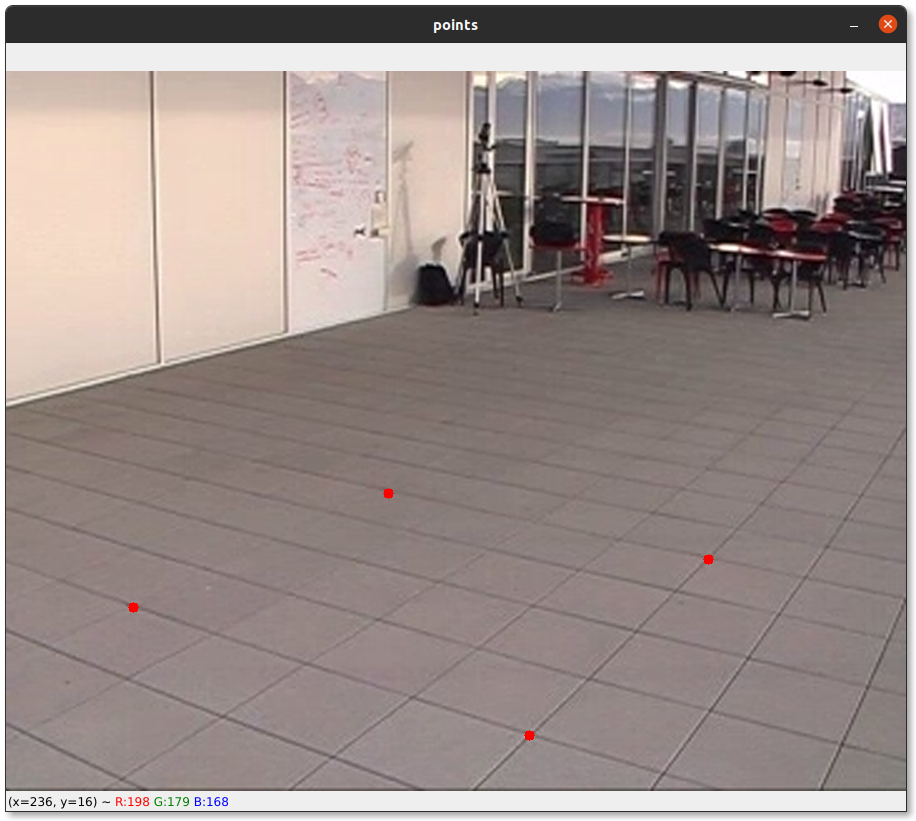
\includegraphics[width=10cm]{images/calibration1.png}
    \caption{Калибровка. Мы выбираем 4 точки квадрата на изображении}
    \label{<label>}
\end{figure}

\begin{figure}[H]
    \centering
    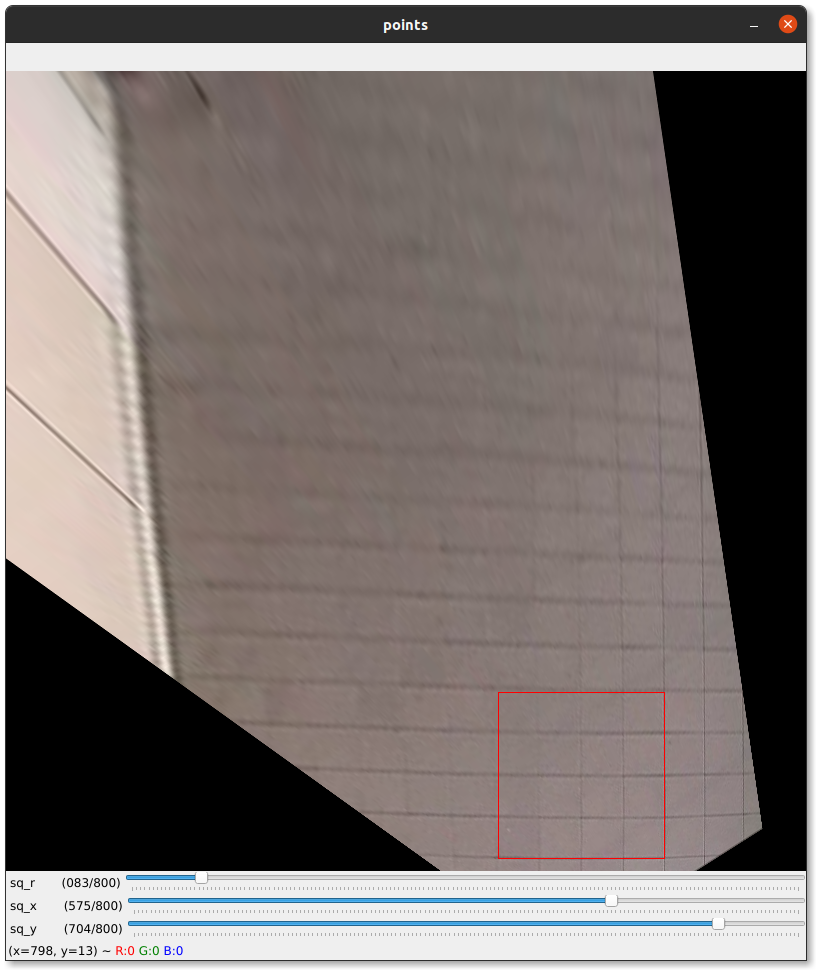
\includegraphics[width=10cm]{images/calibration2.png}
    \caption{Калибровка. Выбираем желаемый масштаб и смещение}
    \label{<label>}
\end{figure}

\begin{figure}[H]
    \centering
    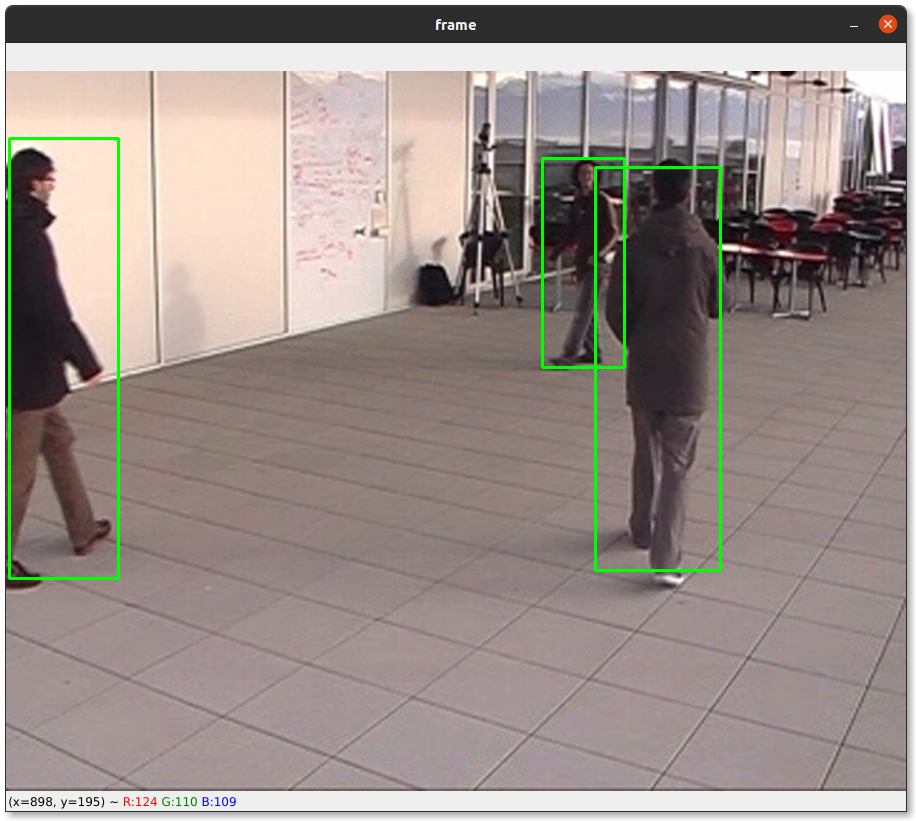
\includegraphics[width=10cm]{images/safe1.png}
    \caption{Зеленым отмечены люди на безопасной дистанции друг от друга}
    \label{<label>}
\end{figure}

\begin{figure}[H]
    \centering
    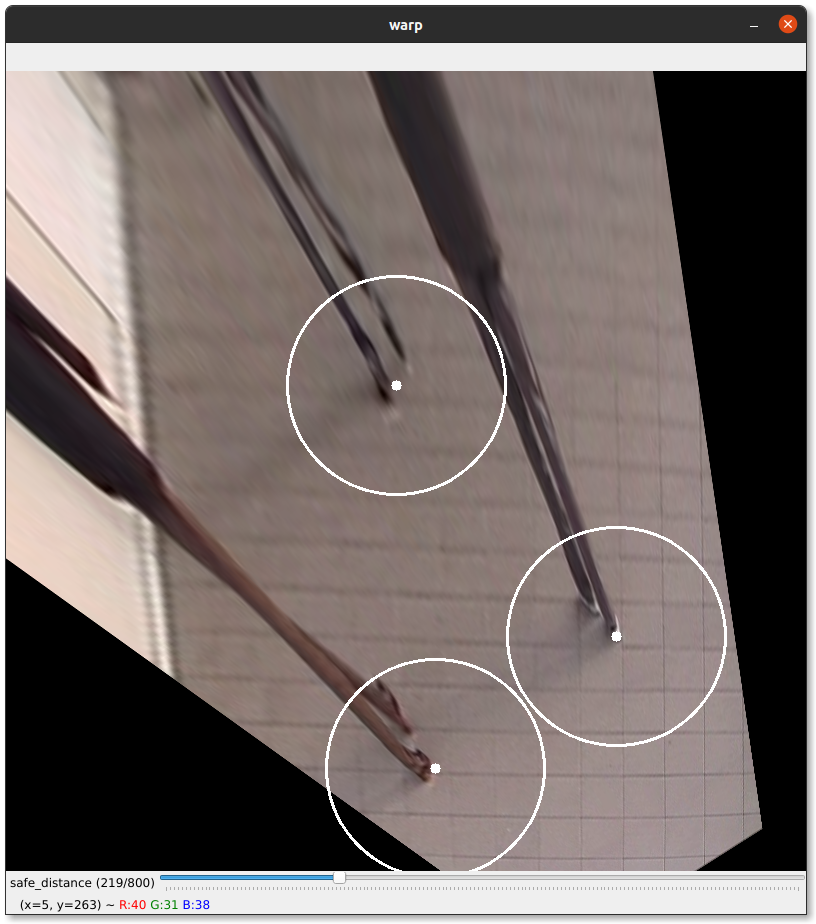
\includegraphics[width=10cm]{images/safe2.png}
    \caption{Вид сверху}
    \label{<label>}
\end{figure}

\begin{figure}[H]
    \centering
    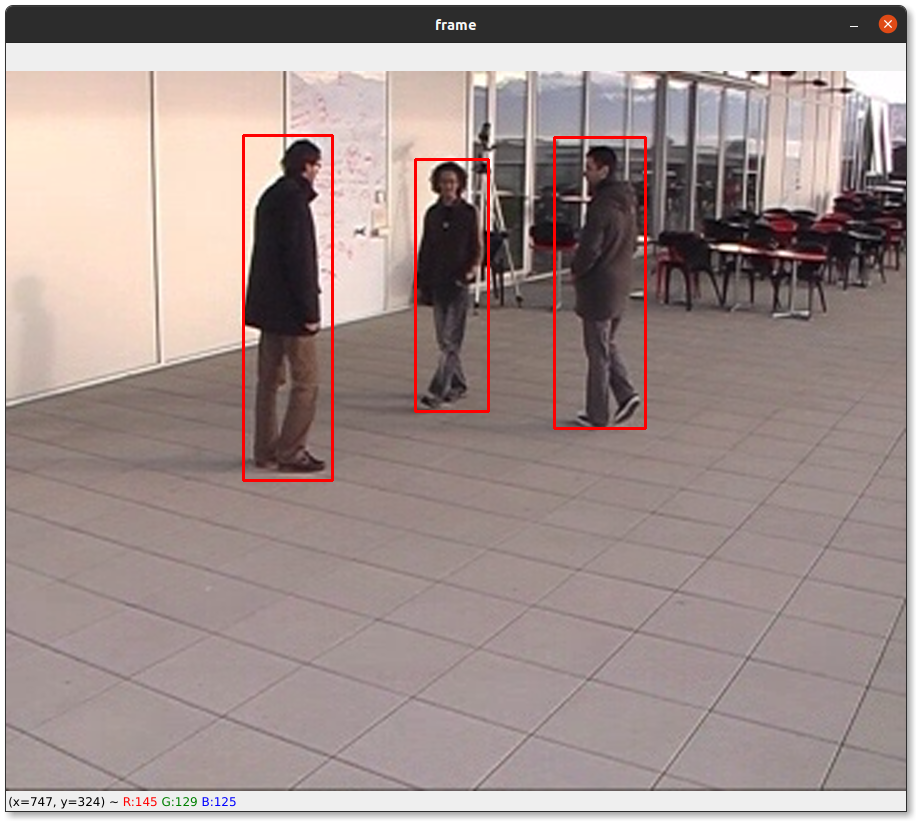
\includegraphics[width=10cm]{images/danger1.png}
    \caption{Красным отмечены люди, нарушающие социальную дистанцию}
    \label{<label>}
\end{figure}

\begin{figure}[H]
    \centering
    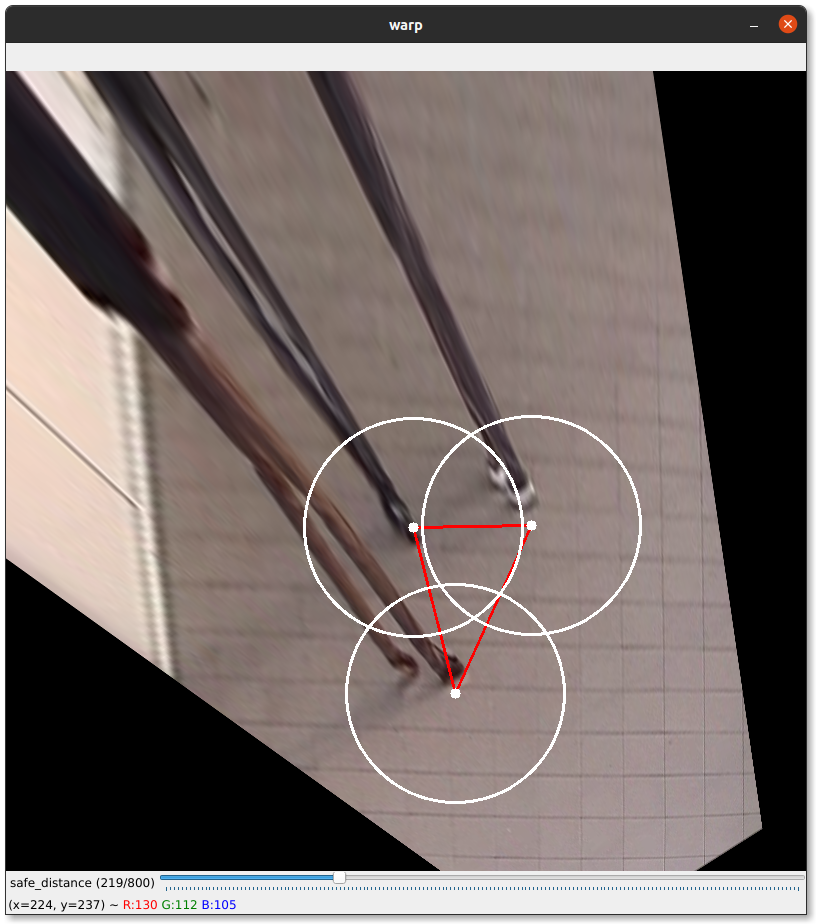
\includegraphics[width=10cm]{images/danger2.png}
    \caption{Вид сверху}
    \label{<label>}
\end{figure}
